\section{Datenübertragung}
Die Datenübertragung erfolgt über 
CAN\footnote{\textbf{C}ontroller \textbf{A}rea \textbf{N}etwork}. Dazu werden 
die Datenleitungen mittels Kondensatoren auf die Busleitungen eingekoppelt. Da 
CAN nicht frei von DC ist, müssen die korrekten Signalpegel wiederhergestellt 
werden. Ohne aktive Kommunikation auf dem Bus liegen beide Datenleitungen auf 
der halben Versorgungsspannung. Diese beträgt typischerweise 5\si{\volt}. 
Somit werden die Datenleitungen mittels Widerständen auf einer Spannung von 
2.5\si{\volt} gehalten. 
\begin{figure}[h!]
    \centering
    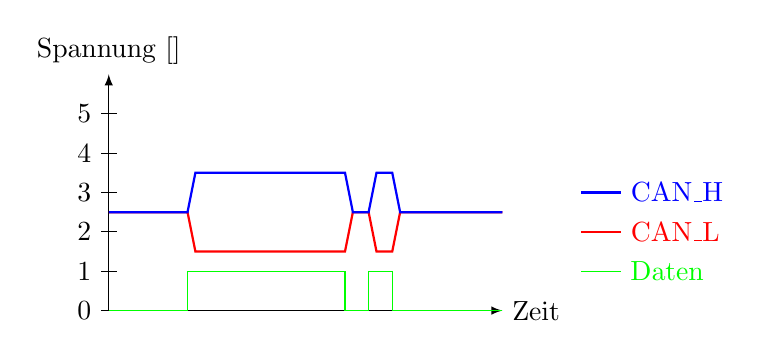
\begin{tikzpicture}
        \draw[-latex] (0,0) -- (5,0) node[right] {Zeit};
        \draw[-latex] (0,0) -- (0,3) node[above] {Spannung [\si{\volt}]};
        \foreach \i in {0,1, ..., 5}
            \draw[] (0.1,\i/2) -- (-0.1,\i/2) node[left] {\i};
        \draw[thin, green]
            (0.0,0.0) --
            (1.0,0.0) --
            (1.0,0.5) --
            (3.0,0.5) --
            (3.0,0.0) --
            (3.3,0.0) --
            (3.3,0.5) --
            (3.6,0.5) --
            (3.6,0.0) --
            (5.0,0.0);
        \draw[thick, red]
            (0.0,1.25) --
            (1.0,1.25) --
            (1.1,0.75) --
            (3.0,0.75) --
            (3.1,1.25) --
            (3.3,1.25) --
            (3.4,0.75) --
            (3.6,0.75) --
            (3.7,1.25) --
            (5.0,1.25);
        \draw[thick, blue]
            (0.0,1.25) --
            (1.0,1.25) --
            (1.1,1.75) --
            (3.0,1.75) --
            (3.1,1.25) --
            (3.3,1.25) --
            (3.4,1.75) --
            (3.6,1.75) --
            (3.7,1.25) --
            (5.0,1.25);
        \draw[thin,  green] (6.0,0.5) -- +(0.5,0.0) node[right] {Daten};
        \draw[thick, red]   (6.0,1.0) -- +(0.5,0.0) node[right] {CAN\_L};
        \draw[thick, blue]  (6.0,1.5) -- +(0.5,0.0) node[right] {CAN\_H};
    \end{tikzpicture}
    \caption{CAN Pegel}
    \label{fig:can_levels}
\end{figure}
Dies kann so realisiert werden. Wird ein "'High"' 
übertragen, wird CAN\_H mit der Versorgungsspannung, CAN\_L mit 0\si{\volt} 
verbunden. Da die Signale kapazitiv gekoppelt sind, nähern sich die Spannungen 
wieder 2.5\si{\volt} an. Somit kann nicht mehr korrekt zwischen "'High"' und 
"'Low"' unterschieden werden. Für die Rekonstruktion der Signalpegel kann man 
sich nun zu Nutze machen, dass bei CAN nach sechs identischen Bit ein 
"'Stopfbit"' gesendet wird. Daher kann eine solche "'High"'-Periode maximal 
sechs Taktzyklen dauern. Danach wird garantiert ein "'Low"' gesendet. Dieses 
muss nun genutzt werden, um die Signalpegel wiederherzustellen. Dabei nutzt 
man die Tatsache, dass der Spannungspegel an CAN\_H immer höher als jener an 
CAN\_L ist. 
\begin{figure}[h!]
    \centering
    \begin{circuitikz}
        \draw
            (0,4) node[left] {Bus\_H} to[C=C, o-] (2,4) to[short, -o] (6,4) node[right] {CAN\_H}
            (0,0) node[left] {Bus\_L} to[C=C, o-] (2,0) to[short, -o] (6,0) node[right] {CAN\_L}
            (2,0) to[sDo, *-*] ( 2,4)
            (4,0) to[R, *-*] (4,2) to[R, *-*] (4,4)
            (4,2) to[V=$V_{offset}$] (6,2) node[sground] {}
        ;
    \end{circuitikz}
    \caption{Signalwiederherstellung mittels Diode und Offsetspannung}
    \label{fig:sol}
\end{figure}
Werden nun über einen längeren Zeitraum "'High"' geschickt, sinkt 
der Signalpegel. Damit sinkt auch der Pegel bei einem "'Low"', womit CAN\_H < 
CAN\_L. Daher können die Signalpegel mit einer idealen Diode zwischen CAN\_H 
und CAN\_L wiederhergestellt werden. 
\begin{figure}[h!]
    \centering
    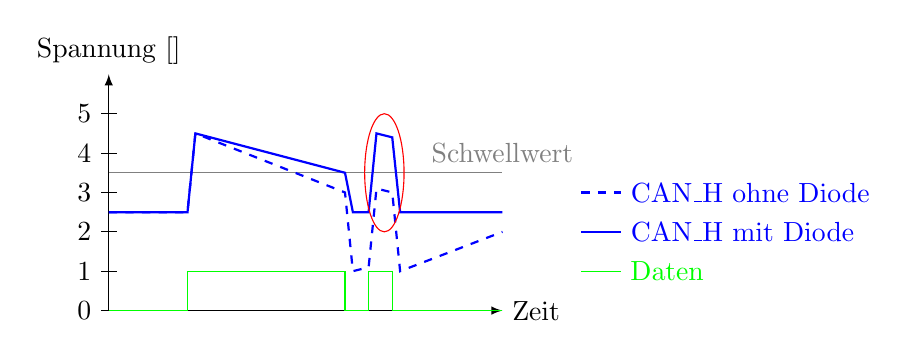
\begin{tikzpicture}
        \draw[-latex] (0,0) -- (5,0) node[right] {Zeit};
        \draw[-latex] (0,0) -- (0,3) node[above] {Spannung [\si{\volt}]};
        \foreach \i in {0,1, ..., 5}
            \draw[] (0.1,\i/2) -- (-0.1,\i/2) node[left] {\i};
        \draw[gray] (0,1.75) -- (5,1.75) node[above] {Schwellwert};
        \draw[thin, green]
            (0.0,0.0) --
            (1.0,0.0) --
            (1.0,0.5) --
            (3.0,0.5) --
            (3.0,0.0) --
            (3.3,0.0) --
            (3.3,0.5) --
            (3.6,0.5) --
            (3.6,0.0) --
            (5.0,0.0);
        \draw[thick, dashed, blue]
            (0.0,1.25) --
            (1.0,1.25) --
            (1.1,2.25) --
            (3.0,1.50) --
            (3.1,0.50) --
            (3.3,0.55) --
            (3.4,1.55) --
            (3.6,1.50) --
            (3.7,0.50) --
            (5.0,1.0);
        \draw[thick, blue]
            (0.0,1.25) --
            (1.0,1.25) --
            (1.1,2.25) --
            (3.0,1.75) --
            (3.1,1.25) --
            (3.3,1.25) --
            (3.4,2.25) --
            (3.6,2.20) --
            (3.7,1.25) --
            (5.0,1.25);
        \draw[thin,  green]        (6.0,0.5) -- +(0.5,0.0) node[right] {Daten};
        \draw[thick, blue]         (6.0,1.0) -- +(0.5,0.0) node[right] {CAN\_H mit Diode};
        \draw[thick, blue, dashed] (6.0,1.5) -- +(0.5,0.0) node[right] {CAN\_H ohne Diode};
        \draw[red] (3.5,1.75) ellipse (0.25 and 0.75);
    \end{tikzpicture}
    \caption{Spannungsverlauf mit und ohne Diode (Nur CAN\_H)}
    \label{fig:can_diode}
\end{figure}
